\section*{Aufgabe 1}
\subsection*{a)} 
Das Integral
\[
I_a = \intbar_{-1}^1 \frac{e^x}{x}\mathrm{d}x
\]
soll numerisch integriert werden.
Dazu lässt sich das Integral umschreiben zu
\begin{align*}
I_a &= \underset{lim}{\epsilon\rightarrow 0}\int_{\epsilon}^1\frac{e^x}{x}\mathrm{d}x + \int_{-1}^{-\epsilon}\frac{e^x}{x}\mathrm{d}x\\
&=\underset{lim}{\epsilon\rightarrow 0}\int_{\epsilon}^1\frac{e^x}{x}\mathrm{d}x - \int_{1}^{\epsilon}\frac{e^-x}{x}\mathrm{d}x\\
&=\underset{lim}{\epsilon\rightarrow 0}\int_{\epsilon}^1\frac{e^x+e^{-x}}{x}\mathrm{d}x
\end{align*}
Wird eine ONC wie etwa die Mittelpunktsregel verwendet, kann der Limes betrachtet werden, da die Funktion nicht an der Singularität ausgewertet werden muss. Es ergibt sich der Wert für das Integral zu
\[
I_a = 2.1145017
\]
mit einem Fehler $<10^{-7}$.
\subsection*{b)}
Die Simpsonregel wird verwendet um das Integral
\[
I_b = \int_0^{\infty} \frac{e^{-x}}{\sqrt{x}} \mathrm{d}x
\]
zu bestimmen. Um die Polstelle zu umgehen kann mithilfe einer Variablentransformation $x=u^2, \mathrm{d}x=2u\mathrm{d}u$
das Integral umschreiben zu 
\[
I_b = \int_0^{\infty} e^{-u^2} \mathrm{d}u
\]
Da eine numerische Integration bis $\infty$ nicht möglich ist, wird bis zu einem oberen Limit $b$ integriert ($I_1$) und zur Fehlerabschätzung ebenfalls das Integral bis $b'$ bestimmt ($I_2$) und die Abweichung $|I_2-I_1|$ bestimmt. Das Ergebnis der Integration und die Abweichung in Abhängigkeit der oberen Grenze $b$ sind in Abb.\ref{fig:1b} und Abb.\ref{fig:1b_err} aufgetragen.
Es zeigt sich, dass bereits für eine kleines $b$ die Abweichung schnell abnimmt und das Integral den Wert
\[
I_b = 1.77245385
\]
annimmt.
\begin{figure}[h!]
\begin{minipage}{0.45\textwidth}
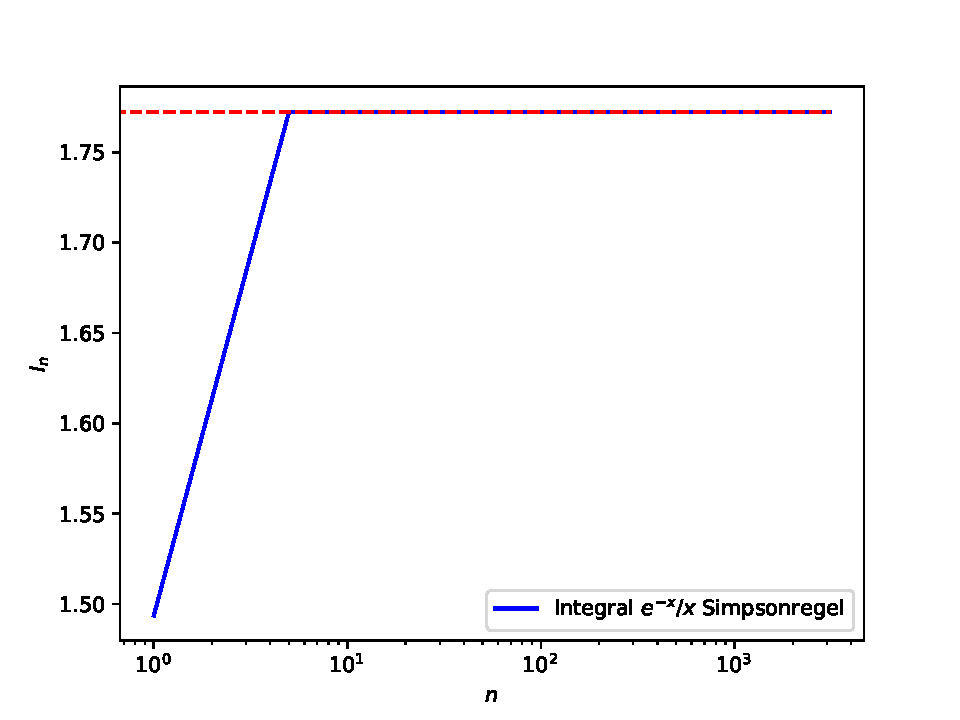
\includegraphics[width=0.9\textwidth]{A1/build/1b.pdf}
\caption{Integralberechnung von $\int_0^{\infty}\frac{e^{-x}}{\sqrt{x}}$ mit Hilfe der Simpsonregel.}
\label{fig:1b}
\end{minipage}
\begin{minipage}{0.45\textwidth}
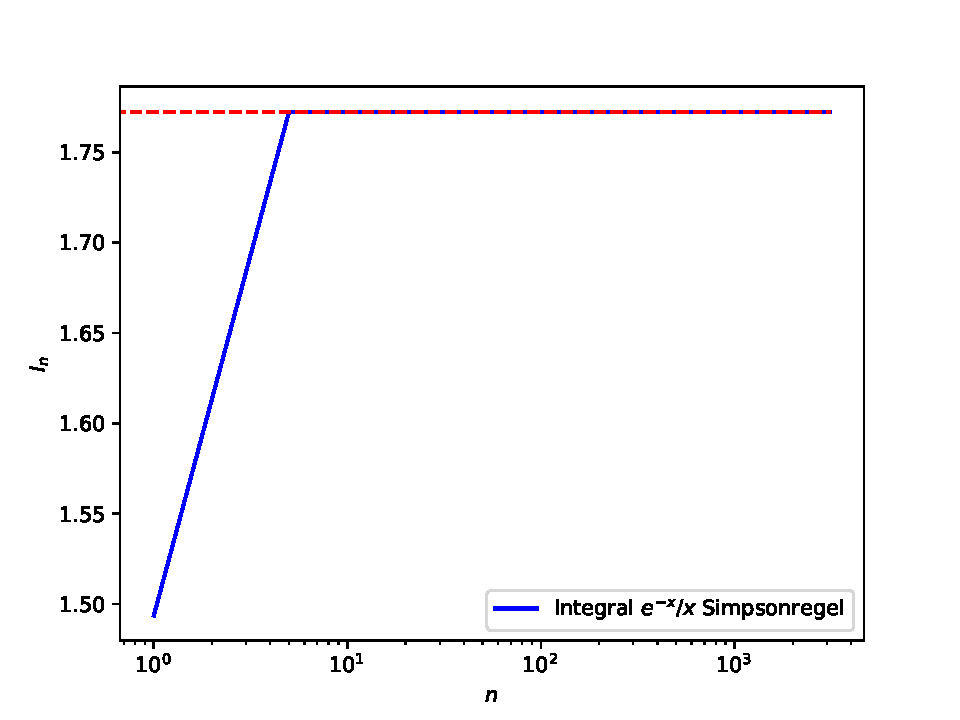
\includegraphics[width=0.9\textwidth]{A1/build/1b.pdf}
\end{minipage}
\end{figure}

